\documentclass{aiaa-tc}

%\usepackage[margin=1.0in]{geometry}
\usepackage{fullpage}
\usepackage{graphicx}
\usepackage{bm} %required for bold in math mode for greek symbols
\usepackage{amsmath} %for bmatrix
\usepackage{amsfonts} %for math script font
\usepackage{url} %for website citations

\usepackage[space]{grffile} %for filepaths with spaces

%define degree symbol:
\newcommand{\degree}{\ensuremath{^\circ}}

\newcommand{\fr}[1]{$#1^+$} %command to write a reference frame
\newcommand{\br}[2]{[#1]_{#2}} %bracket operator with subscript
\newcommand{\tvect}[3]{\begin{bmatrix}#1\\#2\\#3\end{bmatrix}}% 3 x 1 vector
\newcommand{\tvecth}[3]{\begin{bmatrix}#1&#2&#3\end{bmatrix}}% 1 x 3 vector
\newcommand{\B}[1]{\textbf{#1}} %bold for regular vectors
\newcommand{\U}[1]{\hat{\textbf{#1}}} %hats and bold for unit vectors
\newcommand{\BG}[1]{{\bm #1}}           % for vectors using greek letters
\newcommand{\ddt}[1]{\frac{d#1}{dt}} %for time derivatives
\newcommand{\ddarg}[2]{\frac{d#1}{d#2}} % for general derivatives
\newcommand{\pparg}[2]{\frac{\partial#1}{\partial#2}} % for general derivatives
\newcommand{\kron}{\otimes} %redefines \kron to produce kronecker product symbol, for convenience
\newcommand{\squig}[1]{\ensuremath{[{}^{\times} #1]}} % cross product matrix operator

\title{Title}
\author{Tim Woodbury}

\let\endtitlepage\relax %surpress line break after title page

\begin{document}

\maketitle

\section{Rigid body cooperative carry}

The problem is assumed to consist of three rigid bodies; a naturally inert body, labelled body 0, that is to be transported, and quadrotors, which are labelled $i$ and $j$. It is assumed that each quadrotor is tethered to body 0, and that the tether has no slack, although its orientation is not necessarily fixed relative to body 0. If the relative orientations of the tethers and the position of the anchor point on the central body for each tether are known, then the position of each quadrotor relative to the central body is also. The attitudes of the quadrotors are assumed to be unconstrained by the tether. The system has 16 degrees-of-freedom overall; the attitudes of all three bodies (9), the inertial position of any single body (3), and two DOF relating the orientation of each tether to the body (4).

It has been stated that the inertial position of any one body, combined with the knowledge of the tether orientations, is sufficient to localize all three bodies. It is not yet clear whether it is preferable to use the inertial position of the individual quadrotor or the central body, as the former is more natural for vehicle state estimation, but the latter may be more simpler in terms of representing the position of all three bodies. For now, the central body position will be used.

Define the following reference frames: body-fixed reference frames \fr{o}, \fr{i}, and \fr{j} attached to the central body and to quadrotors $i$ and $j$. These frames are assumed to be collocated with the body centers of gravity. In addition, define frames \fr{a_i} and \fr{a_j}; these frames are defined by transformation from \fr{o} such that the 1 axis of \fr{a_i} and \fr{a_j} lies along the vector from the anchor point on the central body to quadrotors $i$ and $j$, respectively. The following values are assumed known: $\br{\B{r}_{ai/o}}{o}$ $\br{\B{r}_{aj/o}}{o}$, the anchor point of the tethers for vehicles $i$ and $j$ relative to the central body center of mass in the central body coordinate system, which is fixed; and the tether lengths $l_i$ and $l_j$. The key position-level variables are:

\begin{itemize}
\item $\B{r}_{o}$: the inertial position of body 0
\item $\B{q}_{o}$: the attitude transformation from the inertial to the body 0 reference frames
\item $\B{q}_{ak}$: the attitude transformation from the body 0 reference frame to the tether $k$ frame, $k \ \in \ \{i,j\}$
\item $\B{q}_{k}$: the attitude transformation from the inertial to the body $k$ reference frames, $k \ \in \ \{i,j\}$
\end{itemize}

The subsequent paragraphs develop, in vector form, the governing kinematic and dynamic equations. $\BG{\omega}_k$ is used to indicate the angular velocity of frame \fr{k} with respect to the inertial reference frame and its time rate in frame \fr{k} is given by ${}^{k}\ddt{\BG{\omega}_k} = \dot{\BG{\omega}}_k$.

In writing the forces acting on each body, a generic quadrotor model with forces and moments $\B{f}^q$ and $\B{l}^q$ is assumed for each vehicle. The tension forces acting on the central body from tethers $i$ and $j$ are denoted $\B{t}_i$ and $\B{t}_j$ and are given in the tether frames by, e.g., $\B{t}_i = t_i \U{a}_{i_1}$. The tension forces are ideal constraint forces and may be omitted in a Kanian or LaGrangian problem formulation. The forces acting on each body are given by:

\begin{align}
\B{f}_0 = \B{t}_i + \B{t}_j - m_0 g \U{n}_1 \\
\B{f}_i = - \B{t}_i + \B{f}^q_i\\
\B{f}_j = - \B{t}_j + \B{f}^q_j
\end{align}

The moments are given by:

\begin{align}
\B{l}_0 = \B{r}_{ai/0} \times \B{t}_i + \B{r}_{aj/0} \times \B{t}_j \\
\B{l}_i = \B{l}^q_i \\
\B{l}_j = \B{l}^q_j
\end{align}

Generally, the position vector to each body is given by:

\begin{align}
\B{r}_0 = \B{r}_0 \\
\B{r}_i = \B{r}_0 + \B{r}_{ai/0} + \B{r}_{i/ai} \\
\B{r}_j = \B{r}_0 + \B{r}_{aj/0} + \B{r}_{j/aj} 
\end{align}

The time rates of the position vectors are:

\begin{align}
\ddt{\B{r}_0} = \B{v}_0 \\
\B{v}_i = \B{v}_0 + \BG{\omega}_0 \times \B{r}_{ai/o} + \BG{\omega}_{ai} \times \B{r}_{i/ai} \\
\B{v}_j = \B{v}_0 + \BG{\omega}_0 \times \B{r}_{aj/o} + \BG{\omega}_{aj} \times \B{r}_{j/aj}
\end{align}

The time rates of the velocity vectors are:

\begin{align}
\ddt{\B{v}_0} = {}^{0}\ddt{\B{v}_0} + \BG{\omega}_0 \times \B{v}_0\\
\ddt{\B{v}_i} = \ddt{\B{v}_0} + \dot{\BG{\omega}}_0 \times \B{r}_{ai/o} + \BG{\omega}_0 \times (\BG{\omega}_0 \times \B{r}_{ai/o}) + \dot{\BG{\omega}}_{ai} \times \B{r}_{i/ai} + \BG{\omega}_{ai} \times (\BG{\omega}_{ai} \times \B{r}_{i/ai}) \\
\ddt{\B{v}_j} = \ddt{\B{v}_0} + \dot{\BG{\omega}}_0 \times \B{r}_{aj/o} + \BG{\omega}_0 \times (\BG{\omega}_0 \times \B{r}_{aj/o}) + \dot{\BG{\omega}}_{aj} \times \B{r}_{j/aj} + \BG{\omega}_{aj} \times (\BG{\omega}_{aj} \times \B{r}_{j/aj})
\end{align}

The attitudes of the three bodies are parameterized independently of one another:

\begin{align}
\dot{\B{q}}_0 = [B(\B{q}_0)]\BG{\omega}_0\\
\dot{\B{q}}_i = [B(\B{q}_i)]\BG{\omega}_i\\
\dot{\B{q}}_j = [B(\B{q}_j)]\BG{\omega}_j\\
\dot{\B{q}}_{ai} = [B(\B{q}_{ai})]\BG{\omega}_{ai}\\
\dot{\B{q}}_{aj} = [B(\B{q}_{aj})]\BG{\omega}_{aj}\\
\B{I}_0 \dot{\BG{\omega}}_0 + \BG{\omega}_0 \times (\B{I}_0 \BG{\omega}_0) = \B{l}_0 \\
\B{I}_i \dot{\BG{\omega}}_i + \BG{\omega}_i \times (\B{I}_i \BG{\omega}_i) = \B{l}_i \\
\B{I}_j \dot{\BG{\omega}}_j + \BG{\omega}_j \times (\B{I}_j \BG{\omega}_j) = \B{l}_j
\end{align}

A minimal set of position coordinates for this problem is: $\br{\B{r}_0}{n}$, $\B{q}_0$, $\B{q}_i$, $\B{q}_j$, $\B{q}_{ai}$, and $\B{q}_{aj}$. (Assumes that each body's attitude is given by a three-parameter set and that $\B{q}_{ai}$ and $\B{q}_{aj}$ are given by two parameters each such as spherical coordinates.)

\subsection{Planar simplification}

Simpler equations of motion can be obtained by considering the planar subproblem. In this case, the position of the mass center of body 0 is given in the inertial frame as $\br{\B{r}_0}{n} = \tvecth{r_{0x}}{r_{0y}}{0}^T$. The location of each anchor $k$ is given by $\br{\B{r}_{ak/0}}{0} = \tvecth{r_{akx}}{r_{aky}}{0}^T$, and $\br{\B{r}_{k/ak}}{n} = l_k\tvecth{\cos{\theta_k}}{\sin{\theta_k}}{0}^T$. We can write inertial-frame position vectors for each body as:

\begin{align}
\br{\B{r}_0}{n} = \tvecth{r_{0x}}{r_{0y}}{0}^T\\
\br{\B{r}_i}{n} = \tvect{r_{0x}}{r_{0y}}{0} + [C_{0/n}^T]\tvect{r_{a1x}}{r_{a1y}}{0} + l_i\tvect{\cos{\theta_i}}{\sin{\theta_i}}{0}
\end{align}

Translational velocity expressions can be derived as follows:

\begin{align}
\br{\B{v}_0}{n} = \tvecth{\dot{r}_{0x}}{\dot{r}_{0y}}{0}^T\\
\br{\B{v}_i}{n} = \tvect{\dot{r}_{0x}}{\dot{r}_{0y}}{0} + [C_{0/n}^T]\squig{\BG{\omega}_0}\tvect{r_{a1x}}{r_{a1y}}{0} + l_i\omega_i \tvect{-\sin{\theta_i}}{\cos{\theta_i}}{0}
\end{align}

The position-level coupling between the three bodies introduces considerable complexity into the resulting expressions. Translational acceleration can be written as:

\begin{align}
\br{\B{a}_0}{n} = \ddt{\br{\B{v}_0}{n}}\\
\br{\B{a}_i}{n} = \ddt{\br{\B{v}_0}{n}} + [C_{0/n}^T]\squig{\BG{\omega}_0}\squig{\BG{\omega}_0}\tvect{r_{a1x}}{r_{a1y}}{0} + [C_{0/n}^T]\squig{\dot{\BG{\omega}}_0}\tvect{r_{a1x}}{r_{a1y}}{0} + l_i\dot{\omega}_i \tvect{-\sin{\theta_i}}{\cos{\theta_i}}{0} + l_i\omega_i^2 \tvect{-\cos{\theta_i}}{-\sin{\theta_i}}{0}
\end{align}

The rotational velocity level states are straightforwardly expressed as $\br{\BG{\omega}_k}{n} = \tvecth{0}{0}{\dot{\lambda}_k}^T$ for $k \ \in \ \{0,i,j\}$, and the angular momentum equations yield $\ddt{\br{\B{h}_k}{n}} = \tvecth{0}{0}{I_k\ddot{\lambda}_k}^T$.

It is assumed that the quadrotor forces and moments may be modelled in the body-fixed frames as:

\begin{align}
\br{\B{f}^q_k}{k} = f_k\U{k}_1 - m_k g \U{n}_1\\
\br{\B{l}^q_k}{k} = l_k\U{k}_3
\end{align}

As presented here, neither a LaGrangian or Kanian approach to obtaining the governing equations of motion offers a simple expression for the development of the translational variables.

%\begin{align}
%gm_0 + gm_i + gm_j + m_0\dot{v}_x + m_i\dot{v}_x + m_j\dot{v}_x - f_i\cos{\lambda_i} - f_j\cos{\lambda_j} - m_i r_{aiy}\dot{\omega}_0 \cos{\lambda_0} - m_j r_{ajy}\dot{\omega}_0\cos{\lambda_0} - li*mi*tidd*sin(thetai) - lj*mj*tjdd*sin(thetaj) - mi*raix*w0d*sin(lambda0) - mj*rajx*w0d*sin(lambda0) - li*mi*tid^2*cos(thetai) - lj*mj*tjd^2*cos(thetaj) - mi*raix*w0^2*cos(lambda0) - mj*rajx*w0^2*cos(lambda0) + mi*raiy*w0^2*sin(lambda0) + mj*rajy*w0^2*sin(lambda0)
%\end{align}

\section{Cooperative localization of moving target}

In this problem, three agents move independently of each other; two cooperating agents and a third, ``target'' agent. The goal of the cooperating agents is for a preselected agent of the pair to reach a specified radius of the target agent. (Aside: this represents nearly identically one of the low-level problems associated with Dr. Rogers's and Clark's coalition research.) 

The dynamics for any individual agent are essentially trivial, and depend only on the choice of model for each. For now, it is assumed that all agents are quadrotors and may move in three dimensional space, but one of the cooperating agents or the target may be restricted to planar motion. The assumed ``goals'' of each agent are:

\begin{itemize}
\item ``Lead'' cooperator: reach a specified radius of the target \\
\item ``Helper'' cooperator: position itself to provide ``good'' or ``optimal'' estimates to the lead \\
\item ``Target'': avoid the lead vehicle for a pre-specified (but possibly unknown) time
\end{itemize}

It is assumed that, although the cooperating vehicles share some or all measurements, a full centralized filter cannot practically be implemented, and each agent must run its own estimator. The key states for estimation for any agent are assumed to be the relative position and velocity vectors of the other two agents. (Depending on the types of vehicles, possible nonholonomic motion constraints may dictate that relative attitude is also highly relevant.) 

At maximum, each vehicle may need to estimate its own position, velocity, and attitude, as well as that of each other vehicle, an 18 DOF problem; however, the states of each vehicle may be decoupled from one another if parameterized as absolute references, or coupled to the estimating vehicle's if parameterized as relative states. The ``optimal'' parameterization will no doubt depend on the sensor measurements available to each vehicle; i.e. a depth sensor such as a laser scanner or RGBD camera provides different information about the target than an RGB camera, and it may be useful in some cases to couple the estimates of other states with the states of the estimating vehicle.

Note that the ``lead'' vehicle may be expected to experience the greatest difficulty localizing the target if range-to-target data are not available (e.g. monoSLAM-like scenario), where the helper vehicle can place itself to increase its parallax to the target and/or the lead agent.

\subsection{2D subproblem}

A restricted subproblem is considered in which all agents move in a plane. This problem is considered for the sake of setting up an example estimator and governing equations.

Each vehicle is assumed to be constrained such that its velocity vector is aligned with the vehicle 1 axis at all times. Each agent estimates is own position and heading relative to an arbitrary inertial frame. (Agents need not use the same inertial frame.) Each agent is assumed to have velocity-level controls for speed and heading angle, allowing the velocity-level states to be treated as controls. To remain as general as practical, standard Cartesian coordinates are used for parameterization. Each agent estimates the position vectors of the other two agents, also parameterized in the inertial frame. For the other cooperating agent, it is assumed that odometry data are shared, enabling filter propagation of the position for that agent. For the target agent, the only available measurements can be relative range and/or bearing. Each agent estimates eight states: position and heading for each cooperating agent, and position of the target agent.

Each agent measures bearing to every other agent, and takes odometry measurements. Odometry, $w_k$, is taken as the distance travelled along the position history of the agent between sample times; it is approximated by summing the norm of the change in position for all numerical integration steps between sample times. It is assumed that the cooperating agents share both of their bearing measurements and odometry, but not control inputs. The bearing measurement of agent $j$ by agent $i$ is denoted $\theta_{ji}$. We can write the measurement model for agent $i$ as:
\begin{align}
w_k = \sum\limits_{j=0}^{M} \| \B{r}_i(t_{j+1}) - \B{r}_i(t_j) \| + v^w_k \ \forall \ \{j : t_{k-1} \leq t_j \leq t_{k}\}, v^w_k \ \sim N(0,\sigma_w^2) \\
\theta_{ji} = \arctan{\frac{r_{jy}-r_{iy}}{r_{jx}-r_{ix}}} - \psi_i \\
\theta_{ti} = \arctan{\frac{r_{ty}-r_{iy}}{r_{tx}-r_{ix}}} - \psi_i
\end{align}

The shared measurements from agent $j$ can be incorporated by flipping the indices in the previous expression. The bearing measurements are directly incorporated into the EKF, giving each agent a total of four measurements per time step. Odometry measurements are treated as inputs to the propagation equations, which allows for reasonable accuracy because of the motion constraint between velocity and heading. The complete propagation equations for agent $i$ are written as:

\begin{align}
\B{r}^i_{k+1} = \B{r}^i_k + \tilde{w}_k \begin{bmatrix}
\cos{\psi^i_k}\\
\sin{\psi^i_k}
\end{bmatrix} - v^w_k\begin{bmatrix}
\cos{\psi^i_k}\\
\sin{\psi^i_k}
\end{bmatrix}\\
\psi^i_{k+1} = \psi^i_k + \omega_i T_s\\
\B{r}^j_{k+1} = \B{r}^j_k + \tilde{w}^j_k \begin{bmatrix}
\cos{\psi^j_k}\\
\sin{\psi^j_k}
\end{bmatrix} - v^{wj}_k\begin{bmatrix}
\cos{\psi^j_k}\\
\sin{\psi^j_k}
\end{bmatrix}\\
\psi^j_{k+1} = \psi^j_k + v^\psi_k, v^\psi_k \sim N(0,T_s^2)\\
\B{r}^t_{k+1} = \B{r}^t_k + v^r_k, v^r_k \sim N(0,(10T_s)^2)
\end{align}

Note that the heading control inputs to agent $j$ and the velocity-level inputs to the target $t$ are assumed unknown; it is assumed that $\omega_j$ is on the order of 1, and the velocity of $t$ is on the order of 10, leading to the variances specified in the preceding equations.

\subsection{Control strategy}

Controls are implemented open-loop with respect to agent estimation, using the true state values. Simple heuristic control strategies are implemented to produce reasonable but suboptimal agent motion. This motion is felt to be relevant even in preliminary simulation. Localizing the target is most difficult in the case when flying directly towards it, which is we assume the pursuit agent will nominally do. Agent 1 denotes the agent tasked with reaching the target. Agent 2 denotes the helper agent. Agent 1 strategy is to move at its maximum speed towards the closest intercept point with the target, assuming the target moves at a known speed along a straight line. At each time step, agent 1 solves for the roots of the following equation with respect to the intercept time $T_{int}$ and the reference heading $\psi_{ref}^1$:

\begin{equation}
0=\B{r}^t_k - \B{r}^1_k + v^t_{max} \begin{bmatrix}
\cos{\psi^t_k}\\
\sin{\psi^t_k}
\end{bmatrix} - T_{int} v^1_{max} \begin{bmatrix}
\cos{\psi^1_{ref}}\\
\sin{\psi^1_{ref}}
\end{bmatrix}
\end{equation}

Depending on the current heading $\psi^1_k$, agent 1 will then turn at the maximum turn rate along the direction that minimizes the heading error. This control strategy is implemented in lieu of solving a free-final time optimal control problem.

Agent 2's objective is to fly relative to agent 1 and the target in a fashion that provides good parallax between both agent 1 observing 2 and agent 2 observing the target. Sequential feedback controllers for agent 2's rate of change of speed $\dot{v}_2$ and turn rate $\omega_2$ are designed to track a reference inertial position. For preliminary investigation, the reference position is taken to be 10 metres from the target along the target's $\pm \U{b}_2$ body-frame axis. The sign of the reference is dictated to place agent 2 on the opposite side of the target from agent 1. Reference heading and velocities are obtained by solving the following equation for $v_{ref}$ and $\psi^2_{ref}$:

\begin{equation}
v_{ref}\begin{bmatrix}
\cos{\psi^2_{ref}}\\
\sin{\psi^2_{ref}}
\end{bmatrix} = -[K](\B{r}^2_k - \B{r}^2_{ref})
\end{equation}

The reference time rates of speed and heading, which are treated as controls,  are given from:

\begin{equation}
\begin{bmatrix}
\dot{\psi}^2_{ref}\\
\dot{v}_{ref}
\end{bmatrix} = 
-[K_v]\left(\begin{bmatrix}
\psi^2_k - \psi^2_{ref}\\
v^2_k - v_{ref}
\end{bmatrix}\right)
\end{equation}

The speed and heading are treated as direct functions of the control inputs, i.e. $\dot{v}^2 = \dot{v}_{ref}$.

The control strategy for the target is simple to drive at its maximum speed along a fixed path. Greater realism could be added by dictating the direction to be orthogonal to the velocity vector of agent 1, for example, but the problem as outlined provides sufficient complexity to examine estimation accuracy.

\begin{figure}
\centering
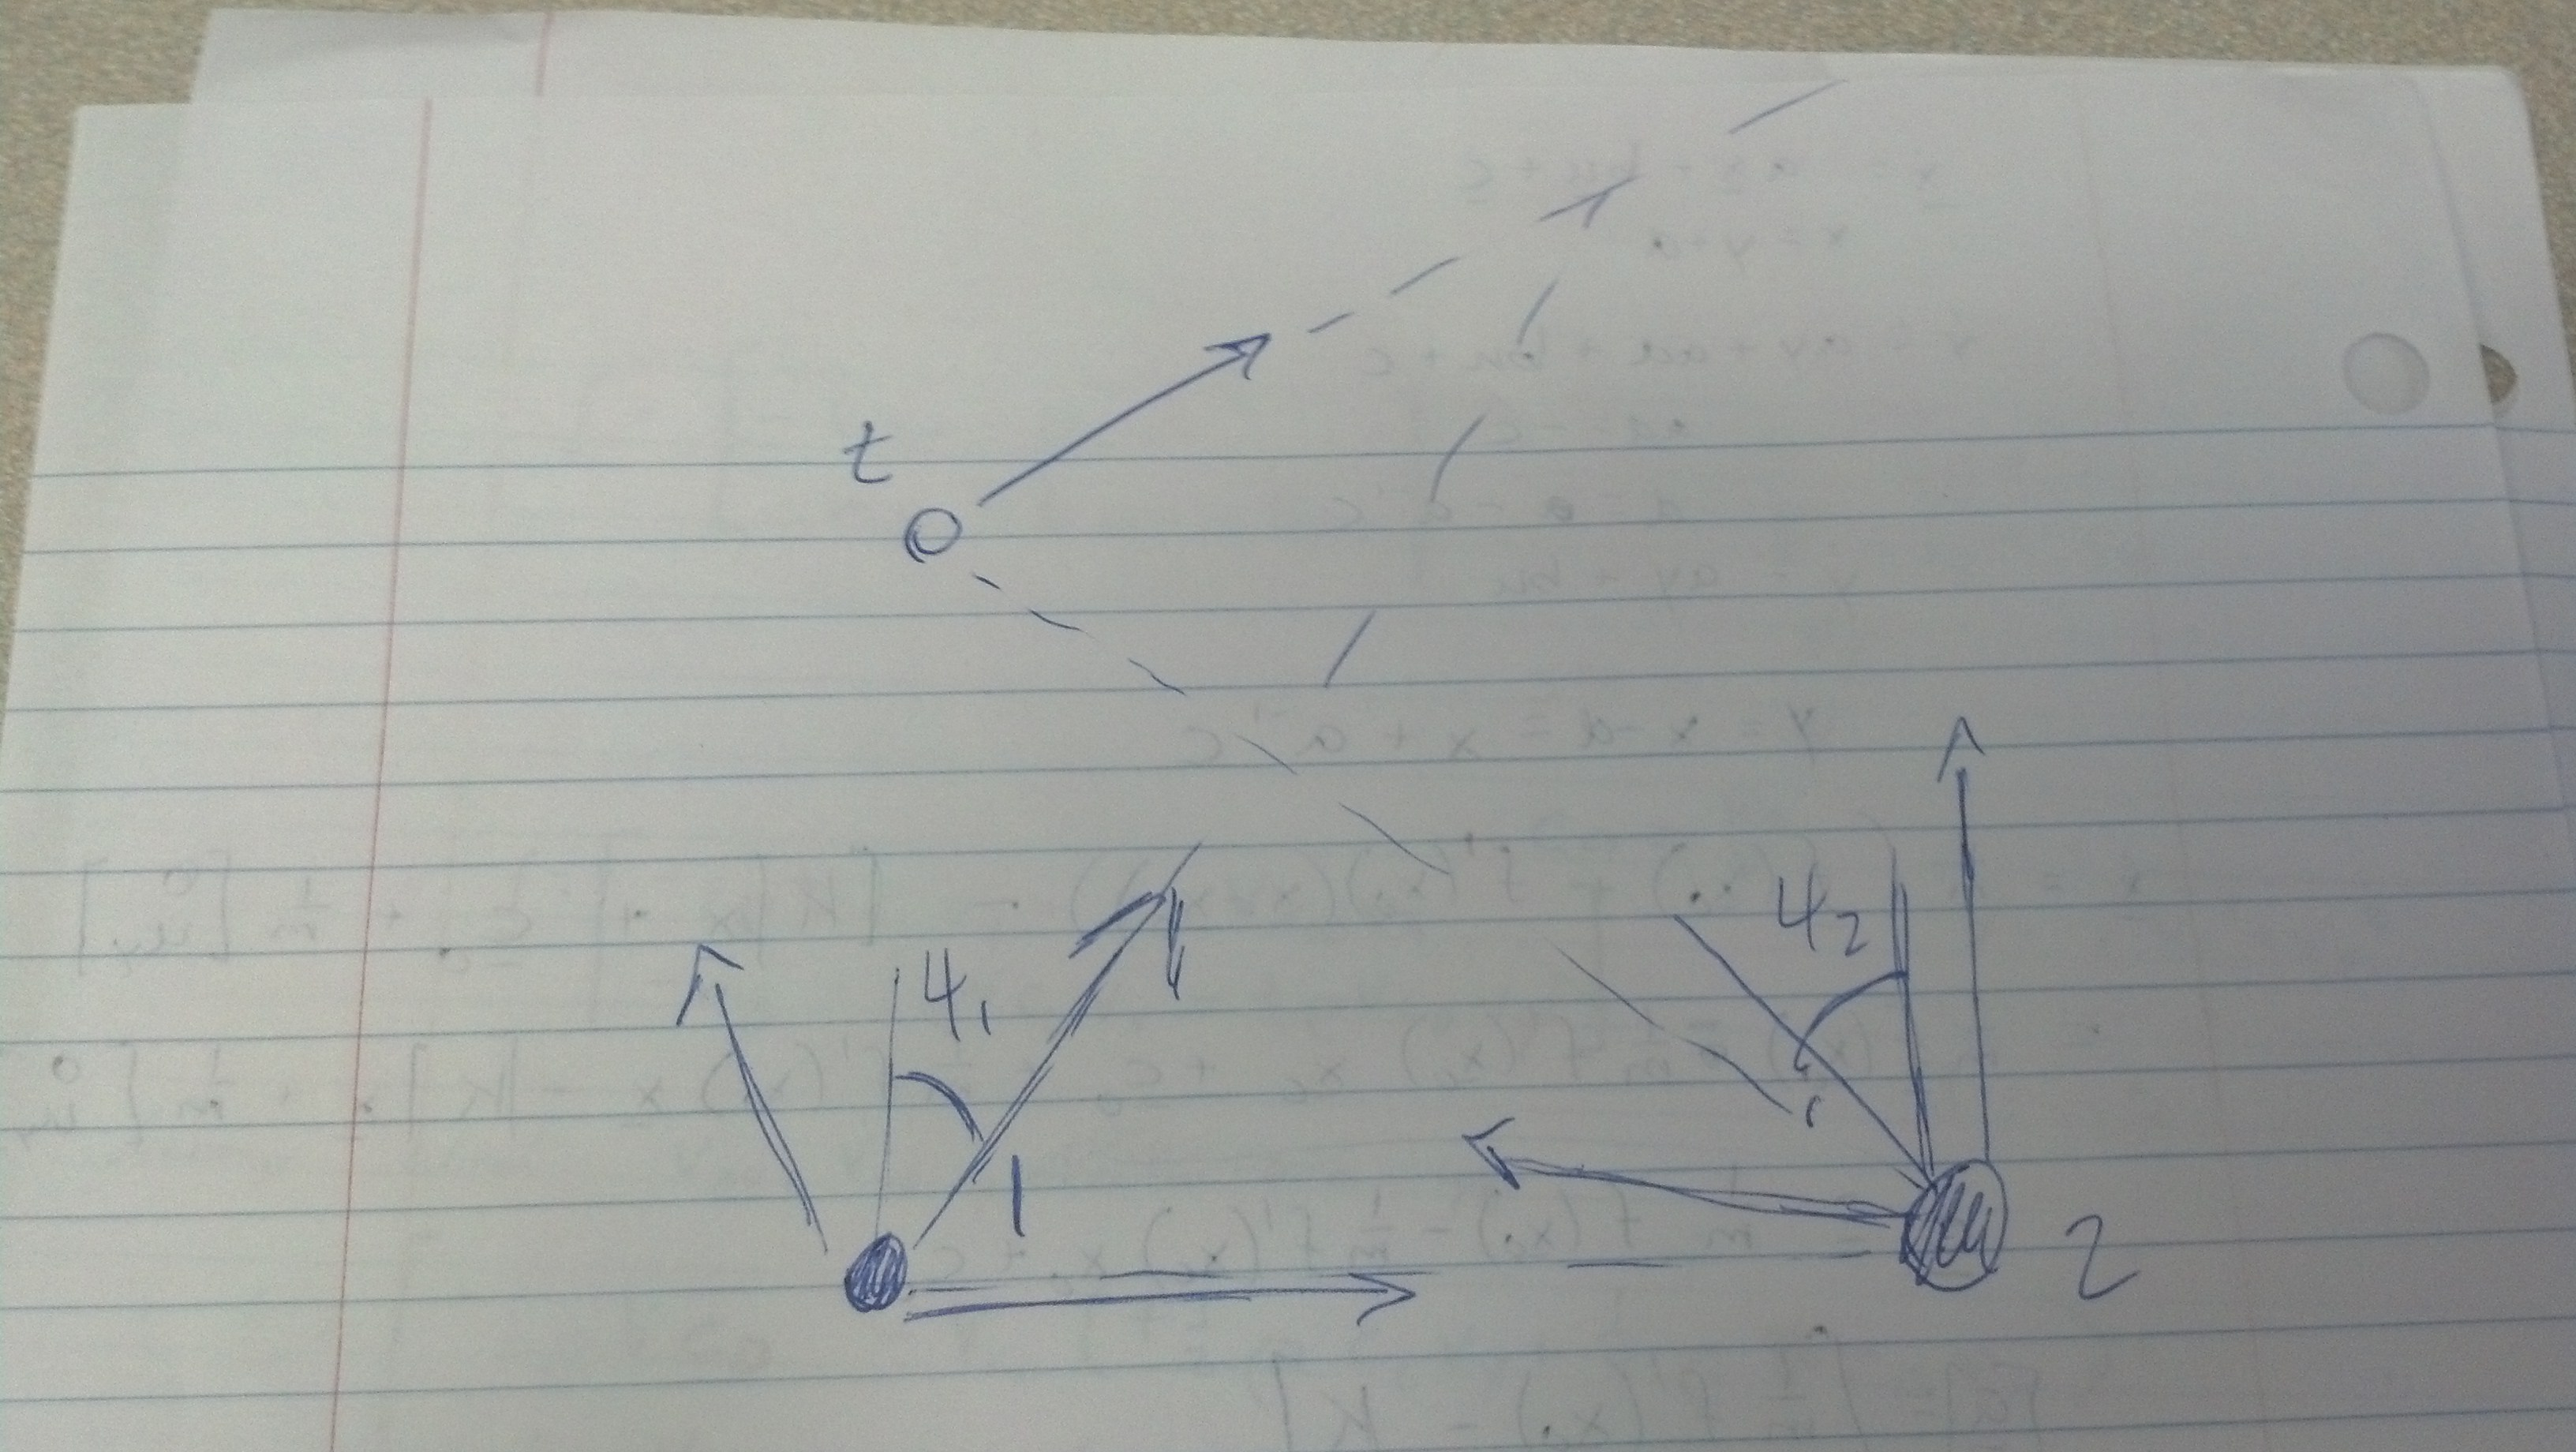
\includegraphics[trim = 250mm 50mm 175mm 50mm,clip = true,width=0.75\textwidth]{target_chase.jpg}
\caption{ Problem geometry showing target $t$, pursuit agent 1, and assisting agent 2.}
\label{fig:target_chase}
\end{figure}

\subsection{Simulation}

Simulation is conducted with a 10 Hz sample rate and the following sensor variances:

\begin{align}
\sigma_\theta^2 = 3.385 \times 10^-5 \\
\sigma_w^2 = .00111 \\
\sigma_{r_t}^2 = 1 \\
\sigma_{\dot{\psi}} = .01
\end{align}

Sensor readings are unbiased. Each agent is initialized in an inertial space where Agent 1 is initially at the origin with zero heading. Agent 2 is initialized at $(5,-5)$ with heading $0.1$ rad. The target is initialized at $(10,0)$ with heading $\pi/4$ rad. The maximum speed of the target is 0.9 m/s. The maximum speed and turn rate of agent 1 is 1 m/s and 1 rad/s. Agent 2's rates are left unconstrained, to ensure it can reach its reference fast enough to provide good measurements, and reach maxima of about 4.5 m/s and 1.3 rad/s. The trajectories are constant for all simulations. Monte Carlo analysis of estimator performance is conducted with new sensor noise and new initial conditions every simulation. The initial estimator states for each vehicle are set between 50\% and 150\% of the true initial states, using a uniformly distributed multiplicative error.

1000 simulations are conducted both using shared measurements and not using shared measurements. Simulation time is 30 seconds each. We concern ourselves mostly with the final range-to-target error for agent 1; the bearing accuracy is relatively low, so range errors will be the most significant source of uncertainty in trajectory generation for agent 1. In 33 simulations, the individual estimator for agent 1 diverges with respect to range-to-target, having a final value of greater than 10 m. Table \ref{tab:mean_std_errs} summarizes errors for the remaining individual cases and for all cooperative cases. Cooperative estimation reduces the standard error by approximately a factor of three. An error bias is not surprising, as the pursuit agent approaches the target along the same trajectory in every simulation.

In examining these results, it should be kept in mind that the agent trajectories are in no way optimized, either for estimation or target tracking purposes. It is also true that SLAM algorithm might be employed to improve localization of the agents and might reduce drift in estimated states. Further, a different parameterization in the filters for the states of the target and/or other agent might produce better results. On the other hand, the trajectories are not closed-loop with respect to the sensing, no effort has been made to address sensor bias, and the agents vary their heading very little for most of the simulation. This exercise is intended to demonstrate the problem and fundamental approach.

\begin{figure}
\centering
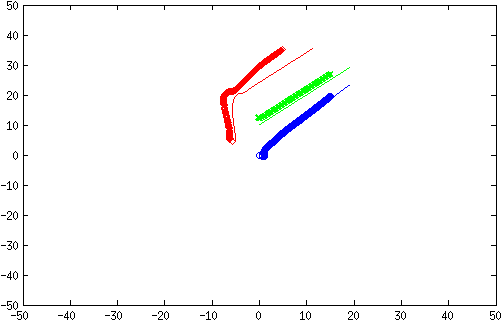
\includegraphics[width=0.75\textwidth]{sample_traj.png}
\caption{ Sample true trajectories (lines) and estimated by agent 2 in one simulation. Target is green, agent 1 is blue, and agent 2 is red. }
\label{fig:sample_traj}
\end{figure}

\begin{table}
\centering
\begin{tabular}{|c|c|c|}
\hline
Case & $\bar{\epsilon}_{\rho_{t1}(t_f)}$ (m) &  $S(\epsilon_{\rho_{t1}(t_f)})$ (m)\\
\hline
Cooperative & 0.686 & 1.13\\
\hline
Individual & 0.783 & 3.69\\
\hline
\end{tabular}
\caption{Mean and standard error associated with agent 1 range-to-target errors at the final simulation time.}
\label{tab:mean_std_errs}
\end{table}

\section{Flexible body cooperative carry}

In this problem, we consider two (or more) agents tasked with jointly transporting a deformable body such as a net or tarp. For simplicity, it is assumed that the deformable body's mass is negligible. The two agents can move freely relative to one another with no new constraint forces relative to normal single-agent motion. An effective kinematic constraint limiting the maximum interagent distance must be considered to avoid an undesireable failure mode. For the sake of safety, a minimum interagent distance should also be introduced to avoid collisions. The problem as posed bears resemblance to the problems of formation flying and collision avoidance in UAVs or satellites.

This problem admits several research challenges, including cooperative navigation and control in the presence of sensor noise and trajectory optimization to improve estimation accuracy. When combined with the cooperative estimation framework, a reasonably complex hardware implementation may be envisioned.

For now, a planar implementation of this problem using the established cooperative estimation framework is considered. This implementation highlights some of the navigation and control challenges that must be addressed.

\subsection{2D subproblem}

Two agents are constrained to move in a plane normal to gravity. These agents may be ground robots or UAVs. Each agent has a limited forward field of view (FOV) sensor that is used to detect features in the environment and perform SLAM or localization in the presence of known features. The agents also measure range and bearing to one another. Agents are tethered by a flexible rope of length $L$ and have a minimum safe distance $D$.

A na\"{\i}ve solution is to have one agent move freely, while the second agent obeys a control law that regulates the interagent distance only. This is one of the simplest conceivable approaches; it ignores any relative heading constraints, and it does not allow direct commands placing the rope in a given orientation in inertial space. Both of these possibilities should be considered in a more realistic implementation. The nai\"{\i}ve controller is used to establish a baseline performance, as well as to explore the research challenges associated with the larger problem.

A Lyanpunov-based nonlinear feedback controller is developed for the follower agent. We consider as the controlled variable the interagent distance $r$ only. Letting the follower agent be designated $i$ and the lead agent be $j$, then we can define $r$ and the radial tracking error $e$ in terms of a reference value $r_{ref}$. The position vectors are componetized in the inertial frame for convenience.

\begin{align}
r = \| \B{r}_j - \B{r}_i \| = \sqrt{ (r_{jx}-r_{ix})^2 + (r_{jy}-r_{iy})^2} \label{eq:rdef} \\
e = r - r_{ref}
\end{align}

Taking the Lyapunov function to be $V = \frac{1}{2} e^2$, we obtain the condition $\dot{e} = -Ke$ as a sufficient condition for stability, $K > 0$. A constant reference $r_{ref} = \frac{L+D}{2}$ is assumed, such that the requirement becomes

\begin{equation}
\dot{r} = -Ke
\end{equation}

Subsituting Eq. \ref{eq:rdef} and isolating for the controlled variables $r_{ix}$ and $r_{iy}$, we obtain the expression:

\begin{equation}
-rKe - ((r_{jx}-r_{ix})\dot{r}_{jx} + (r_{jy} - r_{iy})\dot{r}_{jy}) = \begin{bmatrix}
(r_{ix}-r_{jx}) & (r_{iy}-r_{jy})
\end{bmatrix}
\begin{bmatrix}
\dot{r}_{ix} \\
\dot{r}_{iy}
\end{bmatrix}
\label{eq:outerloop}
\end{equation}

Recognizing the system admits infinitely many control solutions, a minimum-norm solution for $\begin{bmatrix}
\dot{r}_{ix} &
\dot{r}_{iy}
\end{bmatrix}^T$ can be obtained. Compactly representing the system as $A\B{x} = \B{b}$, the minimum-norm solution for \B{x} is $\B{x} = A^T(AA^T)^{-1}\B{b}$. With this minimum-norm solution, Eq. \ref{eq:outerloop} is used to generate reference velocity-level commands.

Similarly, we can define a velocity-level tracking error $\B{e}_v = \B{v} - \B{v}_{ref}$. Using a similar Lyapunov function $V = \frac{1}{2} \B{e}_v^T \B{e}_v$, $\dot{\B{e}}_v = -K_v \B{e}_v$ becomes the condition for stability. Making the assumption that the reference velocity time rates obtained from Eq. \ref{eq:outerloop} are much slower than the dynamics of the velocity states themselves, the control can be reduced to the following form:

\begin{equation}
\begin{bmatrix}
\ddot{r}_{ix} \\
\ddot{r}_{iy}
\end{bmatrix} = -K_v \B{e}_v
\end{equation}

To make the problem interesting, the following agent is modelled as having a thrust-like force in the plane of motion in the direction of its heading. The thrust magnitude and the heading time rate of change are taken as controls. Recalling that the position vectors are componetized in the inertial frame, then a reference heading $\psi$ and thrust command $f_i$ can be obtained:

\begin{align}
f_i\begin{bmatrix}
c\psi \\
s\psi
\end{bmatrix} = -K_v \B{e}_v \\
f_i = \| -K_v \B{e}_v \| \\
\psi = \arctan{ \frac{-\begin{bmatrix}
0 & 1
\end{bmatrix} K_v\B{e}_v}{-\begin{bmatrix}
1 & 0
\end{bmatrix} K_v\B{e}_v }}
\end{align}

The heading rate command is simply taken as the heading error times a high fixed gain. Using the reference thrust and heading, agent 2 is simulated in open-loop using the true state values of agents 1 and 2.

\subsection{Simulation}

The problem is simulated using two agents with bearing-only feature measurements and range and bearing measurements of one another. The feature detection field of view is taken as 130\degree and the agent detection field of view is 360\degree. Agent 1 follows a sinusoidal reference trajectory while Agent 2 uses the control law developed in the previous section with $K = 3.16$ and $K_v = 2.5$. In general, the estimates by Agent 1 behave as expected. For Agent 2, the estimates remain bounded, but generally exceed the 3$\sigma$ covariance estimate. 

Results for one simulation are shown in Figs. \ref{fig:agent1_est}-\ref{fig:agent2_est}. These are typical of results seen in other simulations, although no rigorous Monte Carlo analysis has been performed. The poor estimate accuracy for agent 2 is thought to be caused partly due to frequent and large control excitation, which is not accounted for in the estimator. 

\begin{figure}[p]
\centering
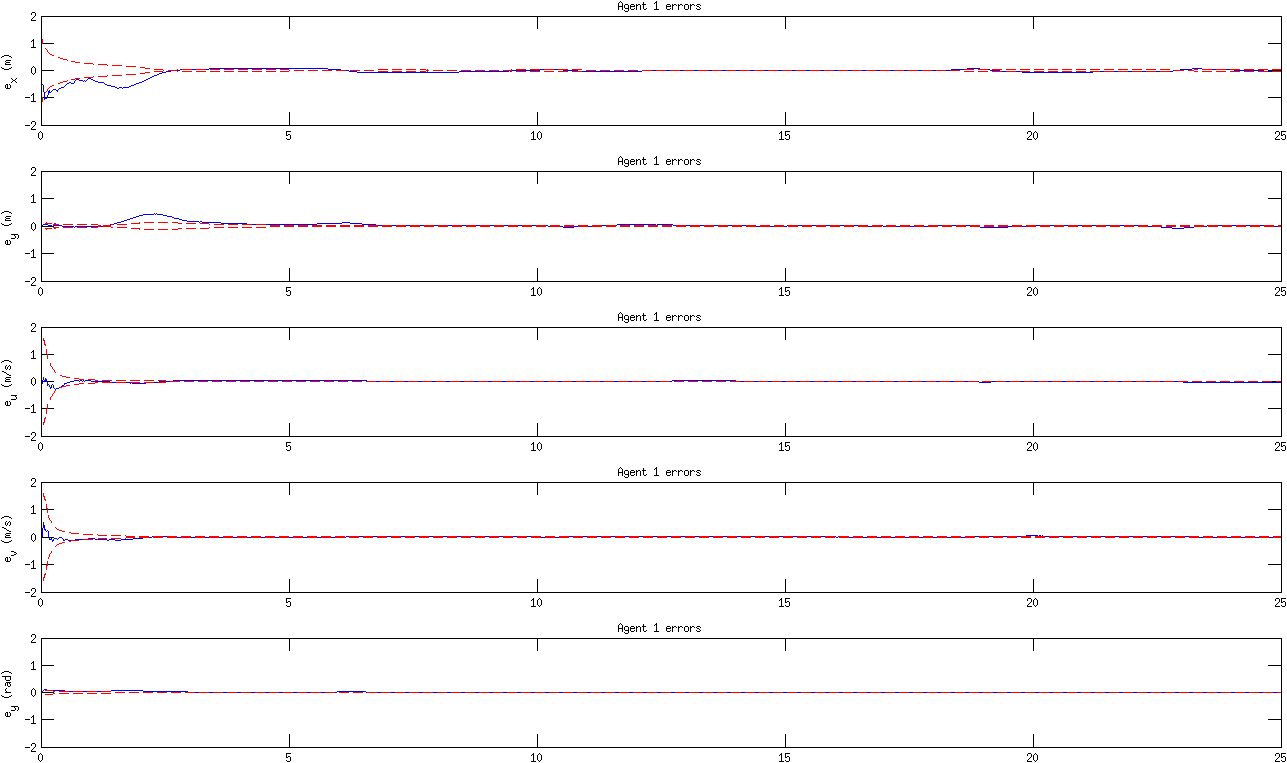
\includegraphics[width=\textwidth]{agent1_est.png}
\caption{ Agent 1 estimate time histories for one simulation. }
\label{fig:agent1_est}
\end{figure}

\begin{figure}[p]
\centering
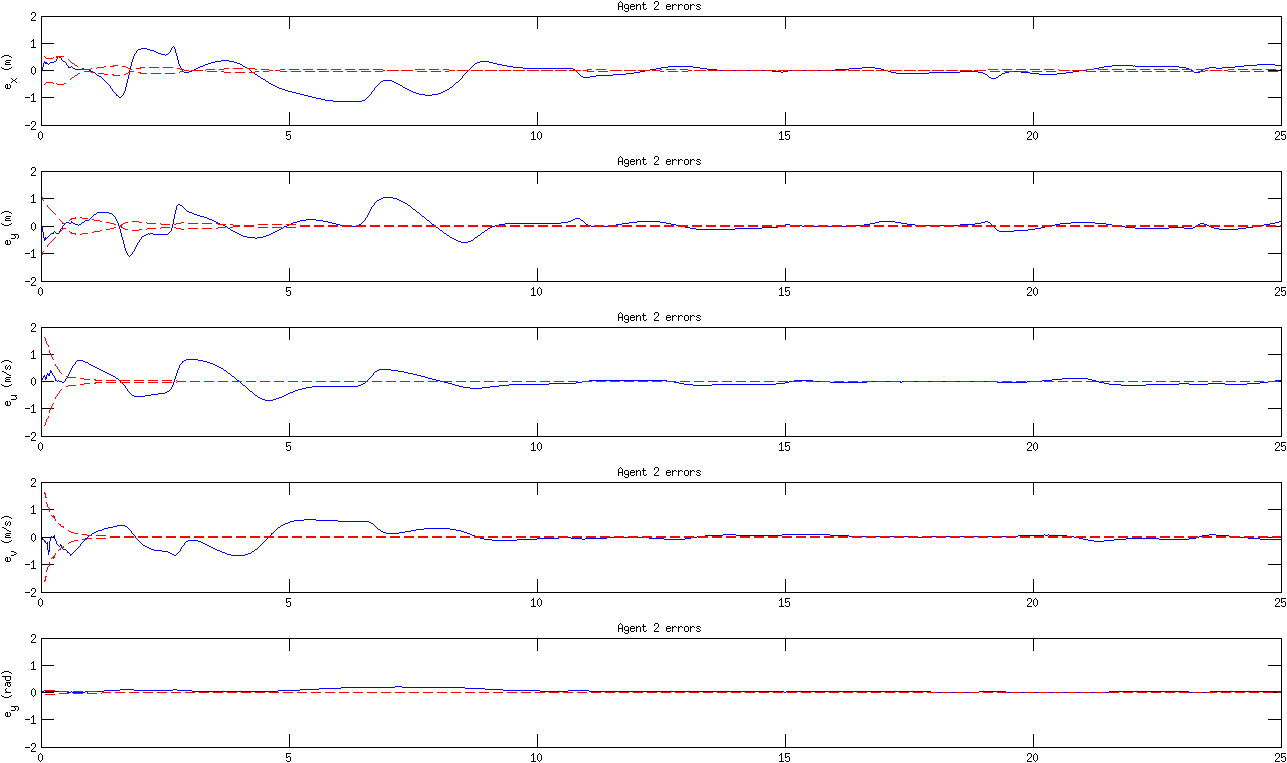
\includegraphics[width=\textwidth]{agent2_est.png}
\caption{Agent 2 estimate time histories for one simulation.}
\label{fig:agent2_est}
\end{figure}

\end{document}
